% Provenance (never printed): see sources/outline_sources.md (Year 2: taphonomy; index fossils;
% facies and fossils as environment markers; reconstructing a palaeoenvironment from a map and a
% section). Taphonomy after Loron (2024); live, dead and fossil assemblages after Tyler and
% Kowalewski (2025); Lagerstaetten after Gaines and others (2024), Mussini and Butterfield
% (2025), Vannier and others (2018), Gerschermann and others (2021) and Rauhut and others
% (2018); zone durations after Al-Suwaidi and others (2022); ichnofacies after Buatois and others
% (2020) and Paz and others (2023); stenohaline groups after McGairy and others (2021) and Saleh
% and others (2022). The Varden column from figdata/shared/region.py; porosities and rates from
% figdata/bachelor-2/palaeoenv.py; exercise and problem values in the Book 4 scratch calculator
% calc/ch20.py. The fossil content given to the Varden units is invented, like the region.
\chapter{Fossielen en paleomilieus}\label{ch:b2:palaeoenvironments}

Op een plaat grijze zandsteen liggen drie aanwijzingen: het spoor dat een trilobiet door de modder ploegde,
de ribbels die een stroming achterliet, en een graafgang die een worm groef en verliet. Geen ervan is een
heel dier, en toch zeggen ze samen dat deze heuvelhelling ooit de bodem van een zee was, ondiep
genoeg om door golven te worden omgewoeld, zout genoeg om er trilobieten in te laten leven. Fossielen zijn de
resten en de sporen van vroeger leven, en geologen lezen ze twee keer: als klokken die het gesteente dateren,
en als getuigen van de plaats waar het ontstond. Dit hoofdstuk volgt een levend wezen van zijn dood
tot de lade van de verzamelaar, opent de zeldzame afzettingen waarin zelfs zachte lichamen overleven, en leest dan
het milieu van een verdwenen zee af, met getallen, in het dek van de Varden Hills.
% ledger: usgs:fossil-record-bulk, loron24:taphonomy

\begin{recall}
\textbf{Uit de schoolboeken}: fossiel, mal, afgietsel en \omterm{def:b2:palaeoenvironments:fossil-kinds}{sporenfossiel}; hoe begraving en mineralen
een schelp tot steen maken; de opeenvolging van fossielen door de tijd. \textbf{Uit Boek~3}:
sedimentaire facies en afzettingsmilieus, turbidieten, riffen en ooïden; biozones,
indexfossielen en eerste-voorkomenshorizonten; compactie, decompactie, de wet van Athy en de vaste dikte
van een laag; cement; accommodatie. \textbf{Uit eerdere hoofdstukken}: transgressies en regressies,
het langetermijnzeeniveau en de \omterm{def:b2:phanerozoic-earth:oae}{oceanische anoxische gebeurtenissen} (\cref{ch:b2:phanerozoic-earth}). Hoe
soorten evolueren, en hoe dieren en planten worden ingedeeld, hoort bij de biologieboeken.
\end{recall}

\section{Van dood tot fossiel}\label{sec:b2:palaeoenvironments:taphonomy}

De meeste levende wezens laten niets achter. Bacteriën en aaseters verteren de zachte delen binnen
dagen of jaren, stromingen breken en verspreiden de harde, en de zuren van bodems en poriewater
lossen op wat overblijft. Een fossiel is wat dit alles overleeft, en daarna nog eens de begraving,
de verhitting en de opheffing van het gesteente dat het bevat.

\begin{definition}[Tafonomie; bewaringspotentieel]\label{def:b2:palaeoenvironments:taphonomy}
\emph{Tafonomie}\index{tafonomie} is de studie van wat er met de resten van een organisme gebeurt
van zijn dood tot zijn ontdekking als fossiel: afbraak, aaseters, transport, begraving, en de
chemische veranderingen van de diagenese. Het \emph{bewaringspotentieel}\index{bewaringspotentieel}
van een organisme, of van een van zijn delen, is de kans dat het deze stadia doorloopt
en in het gesteente bewaard blijft.
\end{definition}
% ledger: loron24:taphonomy

Elk stadium neemt iets weg, voegt iets toe of verandert iets. Afbraak en aaseters verwijderen
zachte weefsels; mineralen uit het poriewater vullen de poriën van een bot of vervangen het aragoniet van een
schelp, en voegen zo materie toe die het dier nooit had; verhitting verandert de organische moleculen die overblijven.
Loron deelt al deze veranderingen na de dood in drie soorten in, winst, verlies en verandering, en
schrijft ze als één vergelijking voor de verandering van elk meetbaar kenmerk tussen een organisme en zijn
fossiel. De figuur hieronder volgt de stadia en wat elk ervan wegneemt.
% ledger: loron24:taphonomy

\begin{omfigure}
\centering
\begin{tikzpicture}[font=\scriptsize, x=1cm, y=1cm,
  stage/.style={draw=black!60, fill=omSea!12, rounded corners=2pt, align=center,
    text width=2.05cm, minimum height=1.25cm, inner sep=2pt},
  loss/.style={align=center, text width=2.05cm, text=omThm!80!black}]
\node[stage] (a) at (0,0) {\textbf{dood}\\een levende\\gemeenschap};
\node[stage] (b) at (2.75,0) {\textbf{afbraak en}\\\textbf{aaseters}\\op de bodem};
\node[stage] (c) at (5.5,0) {\textbf{transport}\\stromingen sorteren\\en breken};
\node[stage] (d) at (8.25,0) {\textbf{begraving}\\onder de\\actieve laag};
\node[stage] (e) at (11,0) {\textbf{diagenese}\\compactie,\\vervanging};
\node[stage] (f) at (13.75,0) {\textbf{blootlegging}\\en\\verzameling};
\foreach \u/\v in {a/b, b/c, c/d, d/e, e/f} {\draw[-{Stealth[length=2mm]}, black!70] (\u) -- (\v);}
\node[loss, anchor=north] at (2.75,-0.8) {zacht weefsel verloren;\\skeletten vallen uiteen};
\node[loss, anchor=north] at (5.5,-0.8) {lichte delen weggevoerd,\\schelpen gebroken};
\node[loss, anchor=north] at (8.25,-0.8) {trage begraving: meer\\tijd voor de verliezen};
\node[loss, anchor=north] at (11,-0.8) {aragoniet opgelost,\\mineralen toegevoegd};
\node[loss, anchor=north] at (13.75,-0.8) {weggeërodeerd,\\of nooit gevonden};
\end{tikzpicture}
\par\smallskip{\small De tafonomische weg van een levende gemeenschap naar een verzameling, met wat
elk stadium wegneemt of verandert. Begraving is het keerpunt: daarvoor staan de resten bloot aan
elk verlies; daarna werken alleen diagenese en erosie erop in.}
\end{omfigure}
% ledger: loron24:taphonomy

De schoolboeken noemden elke rest of elk spoor van vroeger leven dat in gesteente bewaard is een fossiel. De twee soorten
gedragen zich in het gesteente zo verschillend dat ze een eigen naam verdienen.

\begin{definition}[Lichaamsfossiel; sporenfossiel]\label{def:b2:palaeoenvironments:fossil-kinds}
Een \emph{lichaamsfossiel}\index{lichaamsfossiel} is een deel van het lichaam van een organisme, of de mal of het afgietsel
van dat deel: een schelp, een bot, een tand, een blad, en in zeldzame afzettingen een zacht weefsel. Een
\emph{sporenfossiel}\index{sporenfossiel} is een structuur die een organisme door zijn activiteit in of
op een sediment of een gesteente maakte: een voetspoor, een sleepspoor, een graafgang, een boorgat, een voedingspatroon.
\end{definition}

Een \omterm{def:b2:palaeoenvironments:fossil-kinds}{sporenfossiel} maakt deel uit van het sediment waarin het werd gegraven: een stroming die het verplaatste, zou het vernietigen.
Het legt daarom de omstandigheden vast van precies de plaats waar zijn maker leefde, wat een schelp,
die gemakkelijk over de bodem wordt meegerold, niet altijd doet. \omterm{def:b2:palaeoenvironments:fossil-kinds}{Sporenfossielen} krijgen namen zoals organismen, met een
geslacht en een soort, maar de naam beschrijft de structuur, niet het dier: dezelfde graafgang kan
door verscheidene soorten dieren worden gegraven, en één dier kan verscheidene soorten sporen achterlaten.

\subsection*{Begraving tegen vernietiging}

De wedloop tussen begraving en vernietiging kan in een eenvoudig model worden gegoten. Resten die op de
bodem liggen, worden vernietigd met een constante snelheid $k$, de kans per tijdseenheid dat ze worden opgegeten,
gebroken of opgelost; ze zijn veilig zodra een dikte $h$ sediment ze bedekt; en het
sediment hoopt zich op met de snelheid $s$.

\begin{proposition}[Begraving vóór vernietiging]\label{prop:b2:palaeoenvironments:burial}
Onder deze aannamen is de kans dat een rest veilig wordt
\[
  P = e^{-kh/s}.
\]
Ze hangt van de drie grootheden alleen af via de verhouding van de tijd tot begraving, $h/s$, tot
de gemiddelde overlevingstijd op de bodem, $1/k$.
\end{proposition}

\begin{proof}
De rest heeft de tijd $T = h/s$ nodig om door de dikte $h$ te worden bedekt. Met een constante
vernietigingssnelheid $k$ gehoorzaamt de kans $p(t)$ om tot het tijdstip $t$ te overleven aan $p' = -kp$, $p(0) =
1$, zodat $p(t) = e^{-kt}$; bij $t = T$ is dit $e^{-kh/s}$.
\end{proof}

\begin{example}[Een schelp op een rustige bodem]\label{ex:b2:palaeoenvironments:shell}
Veronderstel dat een schelp gemiddeld 20 jaar op de bodem overleeft, $k = \qty{0.05}{yr^{-1}}$, en
veilig is onder $h = \qty{0.1}{m}$ modder. Bij $s = \qty{1}{mm.yr^{-1}}$ is de tijd tot begraving 100
jaar en $P = e^{-5} = 0.0067$: minder dan één schelp op honderd overleeft. Bij
\qty{1}{cm.yr^{-1}} is $P = e^{-0.5} = 0.61$. Een storm die op één dag \qty{0.3}{m} zand afzet,
begraaft alles tegelijk, en dan ligt $P$ dicht bij één. De getallen zijn aangenomen, maar de les
is dat niet: fossielen verzamelen zich waar sediment snel of in plotselinge lagen aankomt.
\end{example}

Het model toont ook waarom het archief vertekend is. Een worm met een zacht lichaam, waarvan de gemiddelde overlevingstijd op
de bodem dagen bedraagt in plaats van decennia, heeft een waarde van $k$ die honderden keren groter is dan die van een dikke
schelp, en dus een exponentieel kleinere kans. Het grootste deel van het fossielenarchief bestaat uit dieren
met schelpen en uit microscopische resten. Tyler en Kowalewski toetsten hoeveel een gemeenschap verliest op
haar weg naar het gesteente. Op 51 plaatsen van een kustzeebodem telden ze 135 levende soorten
ongewervelden, 150 soorten onder de schelpen en skeletten die dood op de bodem lagen, en 112 die
ook een fossielenarchief hebben. De doden zijn talrijker dan de levenden omdat de schelpen op de bodem zich
over vele jaren verzamelden, van dieren die er niet meer leven. Detritivoren en carnivoren, meestal
met een zacht lichaam, worden het minst waarschijnlijk bewaard; toch werden de belangrijkste ecologische groepen van de levende
gemeenschap allemaal teruggevonden onder de doden.
% ledger: usgs:fossil-record-bulk, tyler25:live-dead, tyler25:soft-bodied

\section{Vensters van uitzonderlijke bewaring}\label{sec:b2:palaeoenvironments:lagerstatten}

\begin{definition}[Lagerstätte]\label{def:b2:palaeoenvironments:lagerstatte}
Een \emph{Lagerstätte}\index{Lagerstätte} (meervoud Lagerstätten) is een sedimentaire afzetting die
fossielen van uitzonderlijke kwaliteit bewaart, in het bijzonder de zachte, niet-gebiomineraliseerde weefsels die
afbraak bijna overal elders vernietigt; zo'n afzetting heet ook een Konservat-Lagerstätte.
\end{definition}
% ledger: gaines24:konservat

\omterm{def:b2:palaeoenvironments:lagerstatte}{Lagerstätten} zijn zeldzaam, maar veel van wat over dieren met een zacht lichaam bekend is, komt ervan, en
de eerste grote radiatie van dieren, in het Cambrium, wordt er het best door begrepen.
% ledger: gaines24:konservat

\subsection*{De Burgess Shale}

In 1909 schetste Charles Walcott in zijn veldboek een kleine geleedpotige die hij in de Burgess
Shale van Brits-Columbia had gevonden. Later verzamelde hij er honderden
exemplaren van, \emph{Waptia}, uit één enkel interval van ongeveer \qty{2}{m} dik, het Phyllopod
Bed; de moderne beschrijving ervan berust op meer dan 1800 exemplaren die in twee musea worden bewaard. De Burgess
Shale, ongeveer 508 miljoen jaar oud, werd in dieper water afgezet, tegenover een steile onderzeese
breukwand. Tot zijn fossielen behoren dieren zonder schelp, bewaard als afgeplatte films van koolstof,
vaak hele lichamen. Zo'n bewaring hangt samen met begraving in zuurstofarme modder waarin dieren niet
groeven en die stromingen niet herwerkten: de verliezen van de figuur hierboven werden meteen gestopt.
% ledger: vannier18:waptia, mussini25:burgess

\begin{omfigure}
\centering
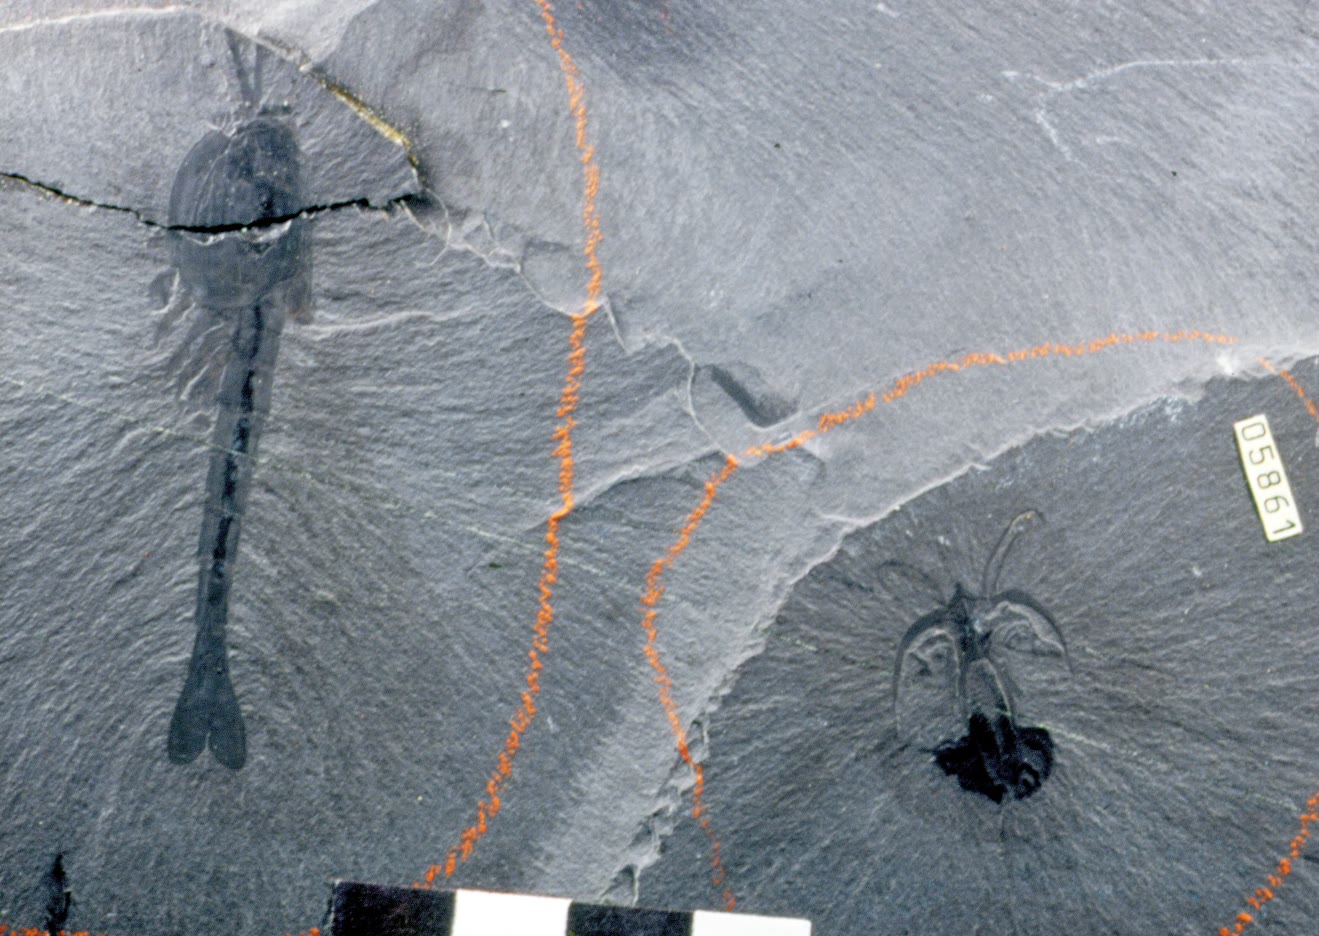
\includegraphics[width=0.72\linewidth]{images/book4/b2-20-burgess-waptia-marrella.jpg}
\par\smallskip{\small Twee geleedpotigen van de Burgess Shale, bewaard als donkere films van koolstof:
\emph{Waptia} (links) en \emph{Marrella} (rechts). (James
St.~John, CC~BY~2.0, via Wikimedia Commons.)}
\end{omfigure}
% ledger: mussini25:burgess

\subsection*{Solnhofen}

De fijnkorrelige kalkstenen van Solnhofen en Eichstätt, in Beieren, werden in lagunes afgezet
vroeg in het Tithonien, de laatste etage van het Jura, die \qty{149.2}{Ma} geleden begon. Ze zijn
de typelocatie van twaalf exemplaren van \emph{Archaeopteryx}, van veel pterosauriërs en van vissen
waarvan de zachte weefsels en zelfs kleurpatronen bewaard zijn. Fossielen zijn er zeldzaam, maar hun
bewaring is uitmuntend. Verscheidene omstandigheden zijn voorgesteld, die misschien samen werkten:
bodemwater dat ongeveer drie keer zo zout was als zeewater of zeer alkalisch, wat de bacteriële
afbraak vertraagt; matten van bacteriën die de kadavers afsloten; zuurstofvrij bodemwater, dat
aaseters weghield; en stormen die het kalkslib opwoelden en de kadavers snel begroeven. Elk
ervan verlengt de overlevingstijd $1/k$ of verkort de tijd tot begraving $h/s$.
% ledger: gerschermann21:solnhofen, rauhut18:archaeopteryx, ics4:jurassic-stages

\begin{omfigure}
\centering
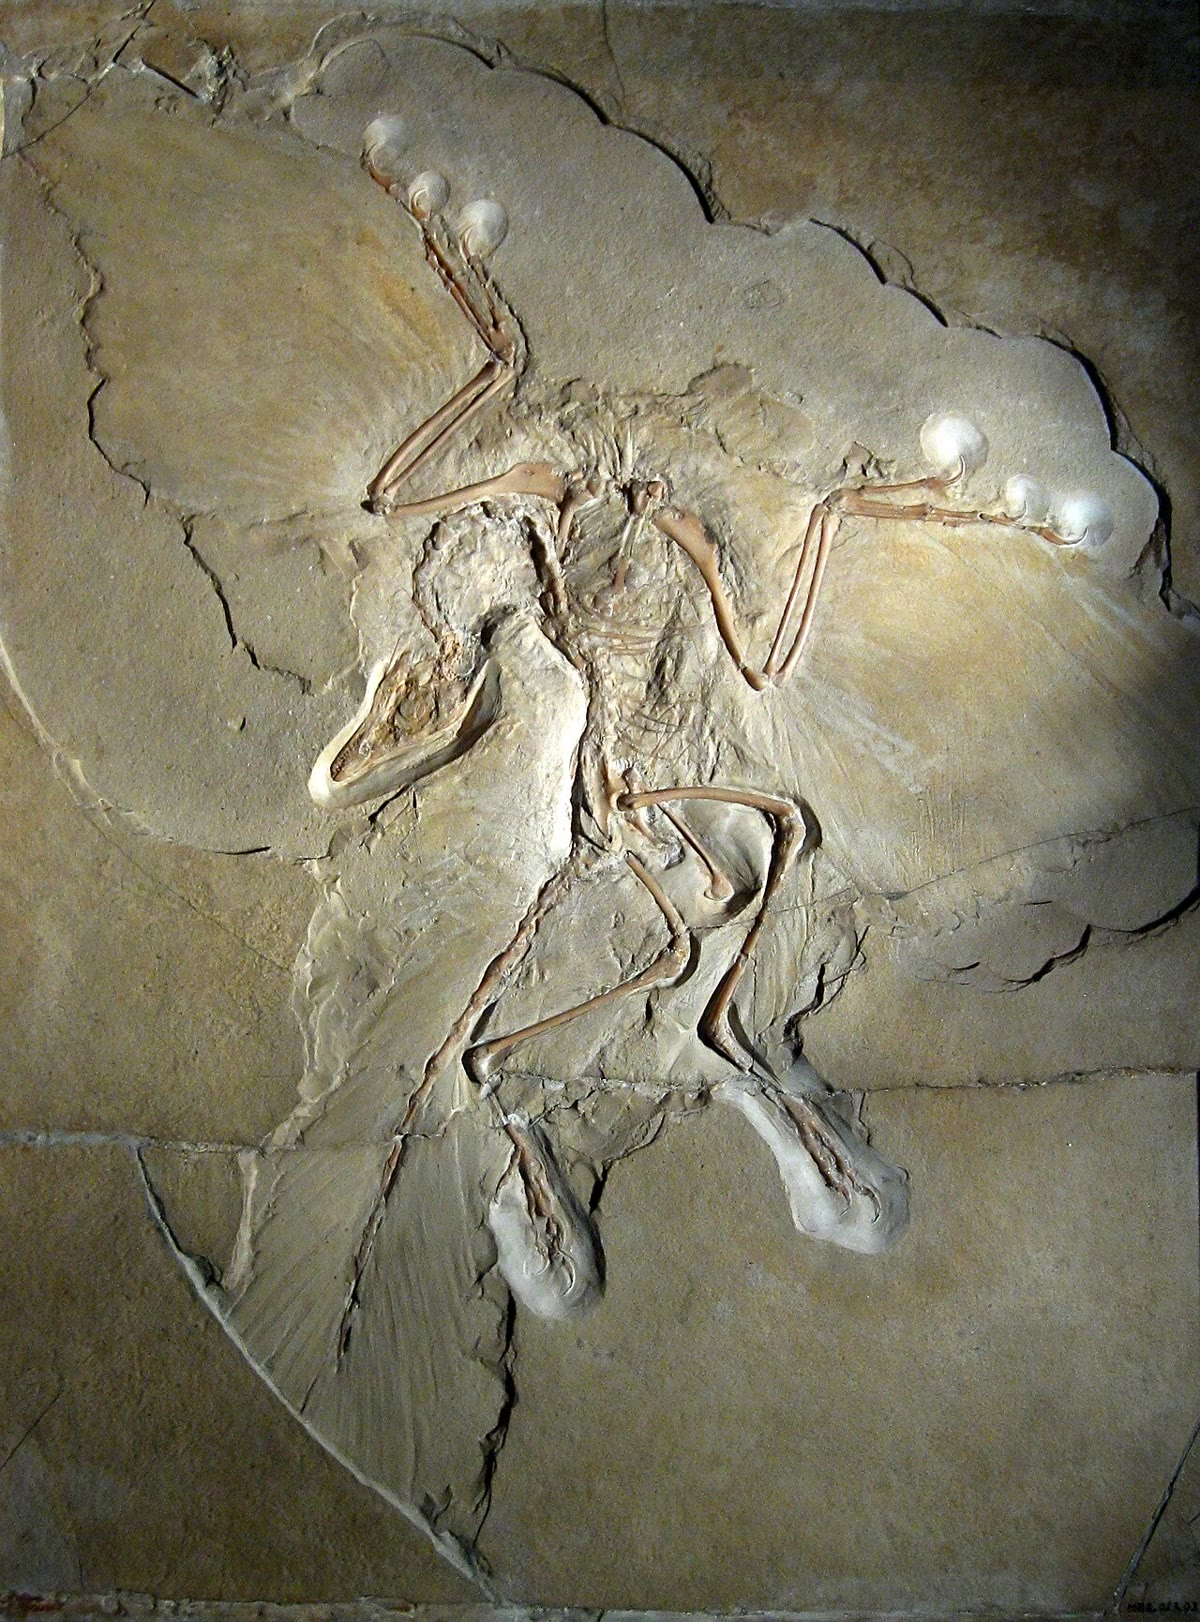
\includegraphics[width=0.5\linewidth]{images/book4/b2-20-archaeopteryx-berlin.jpg}
\par\smallskip{\small Het Berlijnse exemplaar van \emph{Archaeopteryx}, uit de kalkstenen van Solnhofen:
de beenderen en de afdrukken van de veren van vleugels en staart. (H.~Raab, CC~BY-SA~3.0,
via Wikimedia Commons.)}
\end{omfigure}
% ledger: rauhut18:archaeopteryx, gerschermann21:solnhofen

\subsection*{Fossielen als klokken}

Boek~3 bouwde de biozone op, een pakket lagen dat door zijn fossielen wordt gedefinieerd, en het
indexfossiel dat haar herkent. Hoe fijn is de klok die ze vormen? Een ammonietenzone uit het Jura kan
ongeveer een miljoen jaar duren: de vroegste zone van het Toarcien, gedateerd met uranium--loodouderdommen van aslagen in
Argentinië, beslaat 183.73 tot \qty{182.77}{Ma}. Zones worden in horizonten verdeeld, en in het Laat-Jura
duurt een ammonietenhorizont gemiddeld \qty{165}{kyr}. Alle skeletten van
\emph{Archaeopteryx} komen uit één enkele zone die vijf horizonten bevat, dus de vogel is bekend over
zo'n 0.7 tot 1 miljoen jaar. De fossielen geven echter alleen een volgorde; de ouderdommen in jaren komen
van aslagen die met uranium en lood zijn gedateerd, en van sedimentaire cycli. Dezelfde aslagen plaatsen de basis van het Toarcien op $183.73$, met een onzekerheid van
$+0.35$ en \qty{-0.50}{Myr}, waar de internationale kaart \qty{184.2}{Ma} geeft.
% ledger: alsuwaidi22:toarcian, rauhut18:archaeopteryx, ics4:jurassic-stages

\section{Fossielen als getuigen van het milieu}\label{sec:b2:palaeoenvironments:environment}

Om een milieu in een fossiel te lezen, neemt een geoloog aan dat het organisme leefde waar zijn levende
verwanten leven, en dat de processen die vandaag op sediment inwerken toen op dezelfde manier werkten.

\begin{definition}[Actualisme]\label{def:b2:palaeoenvironments:actualism}
\emph{Actualisme}\index{actualisme} is de methode om geologische archieven uit het verleden te interpreteren aan de hand van de
processen, en de relaties tussen organismen en hun milieu, die vandaag kunnen worden waargenomen.
\end{definition}

In 1830 gaf Charles Lyell het eerste deel van zijn \emph{Principles of Geology} de ondertitel ``een
poging om de vroegere veranderingen van het aardoppervlak te verklaren door te verwijzen naar oorzaken die nu
werkzaam zijn''. De methode heeft grenzen. Veel groepen zijn uitgestorven, en hun levenswijze moet worden
afgeleid uit hun vorm en uit het sediment eromheen; en een milieu uit het verleden heeft vandaag misschien
geen exacte tegenhanger.
% ledger: lyell1830:title

\begin{definition}[Paleomilieu]\label{def:b2:palaeoenvironments:palaeoenvironment}
Een \emph{paleomilieu}\index{paleomilieu} is het geheel van fysische, chemische en
biologische omstandigheden die heersten waar en wanneer een gesteente ontstond: de setting, de diepte en
energie van het water, zijn zoutgehalte, temperatuur en zuurstof, de aard van de bodem, en het leven
erop.
\end{definition}

\subsection*{Waar leefde het fossiel?}

De eerste vraag is of de fossielen leefden waar ze liggen.

\begin{definition}[Leef- en doodsassociaties; autochtone en allochtone fossielen]\label{def:b2:palaeoenvironments:assemblages}
Een \emph{leefassociatie}\index{leefassociatie} is een groep fossielen van organismen die samen
leefden, bewaard waar en zoals ze leefden; een \emph{doodsassociatie}\index{doodsassociatie} is
een groep resten die na de dood zijn samengebracht en die organismen van verschillende plaatsen
en verschillende tijden kan mengen. Een fossiel is \emph{autochtoon}\index{autochtoon fossiel} als het
bewaard is waar het organisme leefde, en \emph{allochtoon}\index{allochtoon fossiel} als het
vóór de begraving van elders werd aangevoerd.
\end{definition}

De aanwijzingen zijn die van transport. Schelpen die nog gesloten zijn, een koraal of een gravende tweekleppige in zijn
groeipositie, tere stekels intact, alle leeftijden van een populatie aanwezig: de fossielen zijn
waarschijnlijk \omterm{def:b2:palaeoenvironments:assemblages}{autochtoon}. Losse kleppen gesorteerd op grootte, gesleten en gebroken fragmenten, schelpen
geconcentreerd aan de basis van een gegradeerde laag: ze werden aangevoerd. Een \omterm{def:b2:palaeoenvironments:assemblages}{doodsassociatie} van schelpen, zoals
die op de kustzeebodem hierboven, bevat nog het grootste deel van de gemeenschap, maar ze verzamelt vele jaren
ervan in één laag: haar fossielen zijn over de tijd uitgemiddeld.
% ledger: tyler25:live-dead

\subsection*{Zoutgehalte en zuurstof}

Sommige dieren verdragen alleen het zoutgehalte van de open zee: ze worden stenohalien genoemd. Stekelhuidigen,
koppotigen, koralen en, in het Paleozoïcum, trilobieten zijn typische stenohaliene groepen; hun
aanwezigheid pleit voor normaal zeewater, en hun afwezigheid in een rijke fauna kan ertegen pleiten.
De afzettingen van een silurisch estuarium in Vietnam bevatten plantenresten, visbeenderen, tweekleppigen, slakken
en mosselkreeftjes, maar geen van deze groepen. Stekelhuidigen ontbreken ook in de Chengjiang-biota,
een \omterm{def:b2:palaeoenvironments:lagerstatte}{Lagerstätte} van ongeveer 518 miljoen jaar oud, hoewel ze in \omterm{def:b2:palaeoenvironments:lagerstatte}{Lagerstätten} van de open zee uit het
Cambrium voorkomen: de dieren van Chengjiang leefden voor een delta, waar zoet water het zoutgehalte deed schommelen.
% ledger: mcgairy21:stenohaline, saleh22:echinoderms, saleh22:age

Zuurstof laat zijn sporen na via de gravers. Waar het bodemwater zuurstof bevat, mengen dieren het
sediment en vernietigen ze zijn fijne laminatie; waar het er geen bevat, blijven de laminae bewaard, ontbreken graafgangen
en vormt zich pyriet, zoals in de zwarte schalies van de \omterm{def:b2:phanerozoic-earth:oae}{oceanische anoxische gebeurtenissen} van
\cref{ch:b2:phanerozoic-earth}. Hetzelfde gebrek aan gravers beschermde de kadavers van de Burgess
Shale.
% ledger: mussini25:burgess

\subsection*{Ichnofacies}

\omterm{def:b2:palaeoenvironments:fossil-kinds}{Sporenfossielen} zijn de beste getuigen van de bodem, omdat ze niet werden verplaatst. Hun makers
reageren op de energie van het water, de stevigheid van de bodem, het voedsel en de zuurstof, en dezelfde
associaties van sporen keren door het hele Fanerozoïcum terug.

\begin{definition}[Ichnofacies]\label{def:b2:palaeoenvironments:ichnofacies}
Een \emph{ichnofacies}\index{ichnofacies} is een terugkerende associatie van \omterm{def:b2:palaeoenvironments:fossil-kinds}{sporenfossielen} die
een geheel van milieuomstandigheden weerspiegelt; ze is genoemd naar een kenmerkend spoor.
\end{definition}

Langs een marien profiel, van de kust tot het diepe bekken, volgen vier mariene \omterm{def:b2:palaeoenvironments:ichnofacies}{ichnofacies} elkaar
op (figuur hieronder). De \emph{Skolithos}-ichnofacies, gedomineerd door verticale, cilindrische of
U-vormige woongangen van suspensie-eters, met weinig horizontale sporen, is typisch voor de
vooroever en de onderwateroever. De \emph{Cruziana}-ichnofacies, gedomineerd door de graafgangen van
depositie-eters, met de sporen van grazers, carnivoren en suspensie-eters, is typisch voor de
offshorezone: de bodem tussen de golfbasis bij mooi weer, de diepte waarboven gewone golven
het sediment omwoelen, en de stormgolfbasis, die alleen door stormgolven wordt bereikt. De \emph{Zoophycos}-ichnofacies,
genoemd naar een graafgang die het sediment in schroefvormige lagen rond een centrale
as herwerkt, is typisch voor het plat onder de stormgolfbasis en voor de helling. De \emph{Nereites}-ichnofacies,
met haar regelmatig meanderende, spiraalvormige en netwerkvormige graafgangen, gelezen als de vallen en
tuinen van dieren die weinig voedsel vonden, is typisch voor de diepzee voorbij de platrand. In
brakke baaien en estuaria is een \omterm{def:b2:palaeoenvironments:ichnofacies}{Cruziana-ichnofacies} met weinig soorten de regel.
% ledger: buatois20:ichnofacies, miguez21:ichnofacies, zhang15:zoophycos, buatois25:graphoglyptids, paz23:nereites

\begin{omfigure}
\centering
\begin{tikzpicture}[font=\scriptsize, x=1cm, y=1cm]
% sea and floor (schematic, not to scale)
\fill[omSea!20] (0.6,0) -- (14,0) -- (14,-3.6) -- (11.2,-3.6) -- (9.6,-1.9) -- (6.2,-1.5)
  -- (3.2,-0.9) -- (1.2,-0.15) -- cycle;
\fill[omLithSand!45] (0,0.25) -- (0.6,0) -- (1.2,-0.15) -- (3.2,-0.9) -- (6.2,-1.5)
  -- (9.6,-1.9) -- (11.2,-3.6) -- (14,-3.6) -- (14,-4.3) -- (0,-4.3) -- cycle;
\draw[black!70, line width=0.6pt] (0,0.25) -- (0.6,0) -- (1.2,-0.15) -- (3.2,-0.9) -- (6.2,-1.5)
  -- (9.6,-1.9) -- (11.2,-3.6) -- (14,-3.6);
\draw[omSea!80!black, line width=0.6pt] (0.6,0) -- (14,0);
\node[anchor=south east, omSea!80!black] at (14,0) {zeeniveau};
% wave bases
\draw[dashed, black!60] (2.133,-0.5) -- (14,-0.5) node[anchor=south east, black!70] {golfbasis bij mooi weer};
\draw[dashed, black!60] (4.7,-1.2) -- (14,-1.2) node[anchor=south east, black!70] {stormgolfbasis};
% zonelabels
\node[align=center] at (1.9,0.55) {vooroever,\\onderwateroever};
\node[align=center] at (4.6,0.55) {offshore-\\zone};
\node[align=center] at (8.0,0.55) {plat};
\node[align=center] at (10.5,0.55) {helling};
\node[align=center] at (12.7,0.55) {bekken};
% Skolithos: vertical tubes
\foreach \x in {1.75,1.95,2.15,2.35} {\draw[black!80, line width=0.7pt] (\x,{-0.15-0.375*(\x-1.2)}) -- ++(0,-0.55);}
\node[align=center] at (2.1,-2.15) {\textbf{\emph{Skolithos}}\\verticale buizen};
% Cruziana: horizontal bilobed trails
\foreach \x in {4.0,4.8} {\draw[black!80, line width=0.6pt] (\x,-1.45) .. controls ++(0.2,0.08) .. ++(0.5,0);
  \draw[black!80, line width=0.6pt] (\x,-1.53) .. controls ++(0.2,-0.08) .. ++(0.5,0);}
\node[align=center] at (4.7,-2.35) {\textbf{\emph{Cruziana}}\\voedingsgangen,\\graassporen};
% Zoophycos: spreite arcs
\foreach \r in {0.12,0.22,0.32} {\draw[black!80, line width=0.5pt] (8.0,-2.25) ++(-\r,0) arc (180:360:\r cm and 0.5*\r cm);}
\draw[black!80, line width=0.6pt] (8.0,-2.25) -- (8.0,-1.8);
\node[align=center] at (8.0,-3.05) {\textbf{\emph{Zoophycos}}\\schroefvormige\\lagen};
% Nereites: meander
\draw[black!80, line width=0.6pt, domain=0:2.2, samples=80, smooth] plot (12.0+\x*0.5,{-3.9+0.12*sin(\x*720)});
\node[align=center, anchor=north] at (12.5,-4.35) {\textbf{\emph{Nereites}}\\meanders, netwerken};
\end{tikzpicture}
\par\smallskip{\small De vier mariene \omterm{def:b2:palaeoenvironments:ichnofacies}{ichnofacies} van het model van Seilacher langs een profiel van de
kust tot het diepe bekken, met een schets van een kenmerkend spoor van elk; de diepten zijn niet op
schaal. De sporen reageren meer op energie, voedsel en zuurstof dan op de diepte als zodanig.}
\end{omfigure}
% ledger: buatois20:ichnofacies, miguez21:ichnofacies, zhang15:zoophycos, buatois25:graphoglyptids, paz23:nereites

De diepte werkt niet rechtstreeks. In een diepzeegeul, waar troebelingsstromen sterk zijn, verschijnen verticale
graafgangen van de \omterm{def:b2:palaeoenvironments:ichnofacies}{Skolithos-ichnofacies} ver onder elke golfbasis; en dicht bij een delta, waar zoet
water en modder binnenstromen, zijn de offshoresporen armer dan elders. De makers verplaatsten zich ook
door de tijd: de graafgang \emph{Zoophycos} leefde in het Paleozoïcum op het plat, in het Mesozoïcum op het lagere plat
en de helling, en in het Cenozoïcum in de diepzee. Een \omterm{def:b2:palaeoenvironments:ichnofacies}{ichnofacies} legt de
omstandigheden op de bodem vast, waaruit de diepte alleen wordt afgeleid, en die afleiding moet rekening houden met
de ouderdom van het gesteente.
% ledger: buatois20:ichnofacies, zhang15:zoophycos

\begin{inthefield}[Fossielen laag voor laag tellen]
Een paleontoloog die een milieu reconstrueert uit een sectie, neemt elke laag op met haar
lithologie, dikte en sedimentaire structuren, en daarna haar fossielen: welke groepen, hoeveel,
of schelpen heel of gebroken zijn, gesloten of open, gesorteerd of niet, en in welke positie ze liggen.
\omterm{def:b2:palaeoenvironments:fossil-kinds}{Sporenfossielen} worden vastgelegd waar ze worden gezien, op de laagvlakken en in de verticale wanden,
met de diepte die de graafgangen bereiken. Omdat een schelp kan worden verplaatst maar een graafgang niet, worden de
twee lijsten gescheiden gehouden; het milieu wordt eerst uit de sporen afgelezen, en de \omterm{def:b2:palaeoenvironments:fossil-kinds}{lichaamsfossielen}
worden daarna nagekeken op tekenen van transport.
\end{inthefield}

\begin{omfigure}
\centering
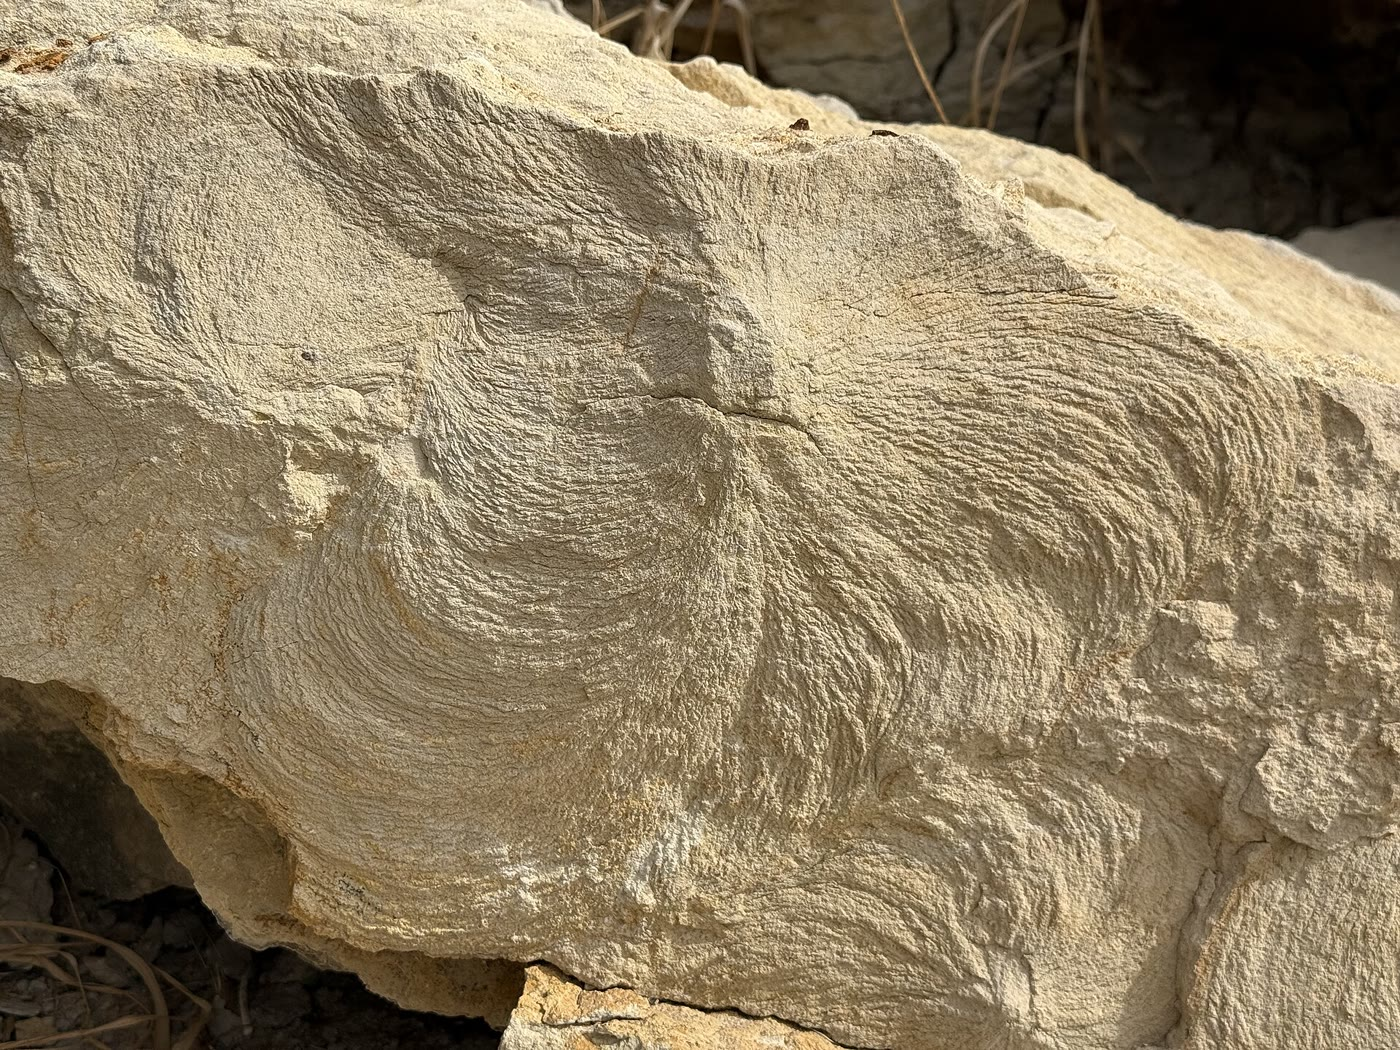
\includegraphics[width=0.5\linewidth]{images/book4/b2-20-zoophycos.jpg}
\par\smallskip{\small \emph{Zoophycos} in een blok bij Sagres, Portugal: de bogen zijn de lamellen
van een schroefvormige laag herwerkt sediment. (Amada44, CC~BY~4.0, via Wikimedia Commons.)}
\end{omfigure}
% ledger: zhang15:zoophycos

\section{Een verdwenen zee lezen}\label{sec:b2:palaeoenvironments:varden}

Milieus liggen naast elkaar: een strand, een offshorebodem, een dieper plat. Wanneer de zee stijgt of
de bodem wegzakt, schuift elk milieu landwaarts over zijn buur, en komen zijn afzettingen
boven op die van de buur te liggen. Een verticale opeenvolging van facies, zonder onderbreking, herhaalt zo
de volgorde van de milieus die naast elkaar lagen; Boek~5 maakt van deze regel,
de wet van Walther, zijn vertrekpunt. Een log die van onder naar boven wordt gelezen, is een film van de kust die
over één plaats trekt.

Het dek van de Varden Hills, het verzonnen gebied van de reeks, vormt een volledig voorbeeld. Zijn
dikten zijn die van het model van het gebied; de fossielen van de figuur hieronder zijn ervoor verzonnen,
maar elk is zo gekozen dat echte gesteenten van die soort het kunnen bevatten. De kalksteen krijgt het
Toarcien, van 184.2 tot \qty{174.7}{Ma}, en de schalie het Aalenien tot het Callovien, van
\qty{174.7}{Ma} tot \qty{161.5}{Ma}.
% ledger: data:b4-palaeoenv, ics4:jurassic-stages

\begin{omfigure}
\centering
% figdata/bachelor-2/palaeoenv.py part log (thicknesses from figdata/shared/region.py)
\begin{tikzpicture}[x=1cm, y=0.0165cm, font=\scriptsize]
% scale
\draw[black!70] (-0.35,0) -- (-0.35,460);
\foreach \z in {0,100,...,400} {\draw[black!70] (-0.45,\z) -- (-0.35,\z) node[left=3pt] {\z};}
\node[rotate=90, anchor=south] at (-1.15,230) {hoogte boven de basis van het dek (m)};
% units
\fill[lith sandstone] (0,0) rectangle (2.2,120);
\fill[lith limestone] (0,120) rectangle (2.0,180);
\fill[lith limestone] (0,180) rectangle (1.6,300);
\fill[lith shale] (0,300) rectangle (1.1,400);
\fill[om lith={icsCretaceous!35}{om limestone}] (0,400) -- (1.4,400) -- (1.4,452)
  .. controls (1.0,466) and (0.6,446) .. (0.3,458) -- (0,455) -- cycle;
\draw[black!70] (0,0) rectangle (2.2,120);
\draw[black!70] (0,120) rectangle (2.0,180);
\draw[black!70] (0,180) rectangle (1.6,300);
\draw[black!70] (0,300) rectangle (1.1,400);
\draw[black!70] (0,400) -- (1.4,400) -- (1.4,452) .. controls (1.0,466) and (0.6,446) ..
  (0.3,458) -- (0,455) -- cycle;
\node[anchor=west, font=\tiny] at (1.45,460) {geërodeerde top};
% unit names
\node[anchor=west, align=left] at (2.6,60) {\textbf{zandsteen}, \qty{120}{m}\\Trias};
\node[anchor=west, align=left] at (2.6,150) {\textbf{oölietkalksteen}, \qty{60}{m}\\Toarcien};
\node[anchor=west, align=left] at (2.6,240) {\textbf{fijne kalksteen}, \qty{120}{m}\\Toarcien};
\node[anchor=west, align=left] at (2.6,350) {\textbf{schalie}, \qty{100}{m}\\Aalenien--Callovien};
\node[anchor=west, align=left] at (2.6,424) {\textbf{krijt}\\Krijt};
% content
\node[anchor=west, align=left, text width=6.9cm] at (6.3,60) {scheefgelaagde geulvullingen op uitgeschuurde
  bases; wortelsporen; plantenfragmenten; geen mariene fossielen};
\node[anchor=west, align=left, text width=6.9cm] at (6.3,150) {scheefgelaagde ooïden; verticale buizen
  en U-vormige graafgangen; gesleten schelpfragmenten};
\node[anchor=west, align=left, text width=6.9cm] at (6.3,240) {stengelleden van zeelelies, brachiopoden,
  belemnieten, ammonieten; kruipsporen en voedingsgangen; lagen van gebroken schelpen met scherpe
  bases};
\node[anchor=west, align=left, text width=6.9cm] at (6.3,350) {donkergrijs, plaatselijk gelamineerd;
  pyriet; ammonieten en dunschalige tweekleppigen; schroefvormige spreitegangen in de lichtere lagen};
\node[anchor=west, align=left, text width=6.9cm] at (6.3,424) {coccolieten; zee-egels, sponzen;
  vuursteenknollen; overal doorgraven};
\foreach \z in {120,180,300,400} {\draw[black!25] (2.25,\z) -- (13.2,\z);}
\node[font=\scriptsize\bfseries, anchor=south west] at (2.6,462) {eenheid en ouderdom};
\node[font=\scriptsize\bfseries, anchor=south west] at (6.3,462) {wat de lagen bevatten};
\end{tikzpicture}
\par\smallskip{\small Het dek van de Varden Hills als log, met de inhoud van zijn eenheden. De
dikten zijn die van het model van het gebied, behalve het krijt, waarvan de geërodeerde top hier is ingekort
(\qty{766}{m} dik in de synclinaal van \cref{ex:b2:palaeoenvironments:shale}); de breedte van de kolom groeit met de korrelgrootte;
de fossielen en hun ouderdommen zijn voor het gebied verzonnen.}
\end{omfigure}
% ledger: data:b4-palaeoenv, ics4:jurassic-stages

\begin{example}[De basis van het dek van de Varden Hills]\label{ex:b2:palaeoenvironments:base}
De zandsteen bevat geulvullingen op uitgeschuurde bases, wortels en plantenfragmenten, en geen enkel marien
fossiel: hij werd door rivieren op het land afgezet. De oölietkalksteen erboven heeft scheefgelaagde ooïden,
die groeien terwijl ze in bewegend water rollen, verticale buizen en U-vormige graafgangen van de \omterm{def:b2:palaeoenvironments:ichnofacies}{Skolithos-ichnofacies},
en gesleten schelpfragmenten, allemaal \omterm{def:b2:palaeoenvironments:assemblages}{allochtoon}: een zandbank van de onderwateroever,
door golven geveegd. Tussen de twee kwam de zee: het contact legt een \omterm{def:b2:phanerozoic-earth:transgression}{mariene transgressie} vast. In
de volgorde van de wet van Walther werd de riviervlakte gevolgd door de kust, en daarna door de zandbank.
\end{example}
% ledger: buatois20:ichnofacies

\subsection*{Hoe snel vulde de zeebodem zich?}

Een biozone geeft een duur, een log geeft een dikte, en hun verhouding is een snelheid. Maar de
dikte is gekrompen sinds het sediment werd afgezet: het water van de poriën is eruit
geperst, en alleen de korrels zijn behouden.

\begin{proposition}[Accumulatiesnelheid van een gecompacteerde laag]\label{prop:b2:palaeoenvironments:rate}
Een laag met huidige dikte $h$ en gemiddelde porositeit $\varphi$, afgezet over de tijd $\Delta t$
met de porositeit $\varphi_0$, hoopte zich op met de snelheid
\[
  r = \frac{h\,(1 - \varphi)}{(1 - \varphi_0)\,\Delta t}
\]
aan vers sediment, en met de snelheid $h(1-\varphi)/\Delta t$ aan korrels, die niet afhangt van
$\varphi_0$.
\end{proposition}

\begin{proof}
Per oppervlakte-eenheid bevat de laag het korrelvolume $h(1 - \varphi)$, de vaste dikte uit
Boek~3. Compactie drijft water uit maar voegt geen korrels toe en neemt er geen weg, dus het verse
sediment, met porositeit $\varphi_0$, had de dikte $h_0$ met $h_0(1 - \varphi_0) = h(1 -
\varphi)$. Door $h_0$ en de vaste dikte door $\Delta t$ te delen, vindt men de twee snelheden.
\end{proof}

Wanneer de porositeit niet werd gemeten, geeft de wet van Athy ze uit de diepte. De figuur hieronder toont
de wet voor vier lithologieën, en de factor $(1 - \varphi(z))/(1 - \varphi_0)$ waarmee een dunne
laag die nu op de diepte $z$ ligt, moet worden uitgerekt om haar dikte aan het oppervlak te geven. Krijt en schalie
beginnen met veel water en verliezen het snel: een dunne laag schalie op \qty{1000}{m} was bij haar afzetting 1.68 keer
zo dik, een laag krijt 2.19 keer.
% ledger: pybacktrack:compaction, pybacktrack4:limestone, data:b4-palaeoenv

\begin{omfigure}
\centering
% figdata/bachelor-2/palaeoenv.py parts poro and ratio
\begin{tikzpicture}
\begin{groupplot}[group style={group size=2 by 1, horizontal sep=1.6cm},
  width=0.46\linewidth, height=6.2cm, y dir=reverse, ymin=0, ymax=3000,
  tick label style={font=\scriptsize}, label style={font=\small}, xtick pos=bottom,
  ytick pos=left, scaled y ticks=false, yticklabel style={/pgf/number format/1000 sep={\,}}]
\nextgroupplot[xmin=0, xmax=0.75, xlabel={porositeit $\varphi$}, ylabel={diepte $z$ (\unit{m})},
  legend style={at={(0.5,1.04)}, anchor=south, draw=none, font=\scriptsize, legend columns=2}]
\addplot[omThm, line width=1pt] table[x=shale, y=z_m] {figdata/out/bachelor-2-palaeoenv-poro.dat};
\addlegendentry{schalie}
\addplot[omSea!80!black, line width=1pt, dashed] table[x=sandstone, y=z_m] {figdata/out/bachelor-2-palaeoenv-poro.dat};
\addlegendentry{zandsteen}
\addplot[black, line width=1pt, dotted] table[x=chalk, y=z_m] {figdata/out/bachelor-2-palaeoenv-poro.dat};
\addlegendentry{krijt}
\addplot[green!45!black, line width=1pt, dash dot] table[x=limestone, y=z_m] {figdata/out/bachelor-2-palaeoenv-poro.dat};
\addlegendentry{kalksteen}
\nextgroupplot[xmin=1, xmax=3.2, xlabel={herstelfactor $(1-\varphi)/(1-\varphi_0)$}]
\addplot[omThm, line width=1pt] table[x=shale, y=z_m] {figdata/out/bachelor-2-palaeoenv-ratio.dat};
\addplot[omSea!80!black, line width=1pt, dashed] table[x=sandstone, y=z_m] {figdata/out/bachelor-2-palaeoenv-ratio.dat};
\addplot[black, line width=1pt, dotted] table[x=chalk, y=z_m] {figdata/out/bachelor-2-palaeoenv-ratio.dat};
\addplot[green!45!black, line width=1pt, dash dot] table[x=limestone, y=z_m] {figdata/out/bachelor-2-palaeoenv-ratio.dat};
\end{groupplot}
\end{tikzpicture}
\par\smallskip{\small Links: porositeit tegen diepte volgens de wet van Athy, met de constanten van Sclater
en Christie (1980) voor schalie, zandsteen en krijt en van Turer en Maynard (2003) voor kalksteen,
zoals getabelleerd in pyBacktrack. Rechts: de factor waarmee een dunne laag op de diepte $z$ wordt
hersteld tot haar dikte aan het oppervlak.}
\end{omfigure}
% ledger: pybacktrack:compaction, pybacktrack4:limestone, data:b4-palaeoenv

\begin{example}[De schalie van de Varden Hills]\label{ex:b2:palaeoenvironments:shale}
In de synclinaal van de Varden Hills is het krijt \qty{766}{m} dik, dus de schalie ligt tussen
766 en \qty{866}{m}. Met de constanten van schalie, $\varphi_0 = 0.63$ en $\lambda =
\qty{1960}{m}$, is de vaste dikte (Boek~3) gelijk aan $100 - 0.63 \times 1960 \times
(e^{-766/1960} - e^{-866/1960}) = \qty{58.4}{m}$, een gemiddelde porositeit van 0.416. Met dezelfde korrels naar het
oppervlak teruggebracht, is de laag \qty{148.6}{m} dik. Over de \qty{13.2}{Myr} van
de basis van het Aalenien tot de top van het Callovien hoopte de schalie zich op met $100/13.2 =
\qty{7.6}{m}$ per miljoen jaar zoals ze nu is, met $148.6/13.2 = \qty{11.3}{m}$ per miljoen
jaar aan verse modder, en met \qty{4.4}{m} per miljoen jaar aan korrels. De huidige dikte
onderschat de snelheid met een derde.
\end{example}
% ledger: data:b4-palaeoenv, pybacktrack:compaction, ics4:jurassic-stages

De schalie heeft misschien ooit nog dieper gelegen, onder krijt dat sindsdien is weggeërodeerd; de correctie is dan een
minimum. Het weekendprobleem past de propositie toe op de kalksteen, waar de porositeit werd
gemeten.

\section*{Oefeningen}\label{sec:b2:palaeoenvironments:exercises}

Gegevens voor de oefeningen, tenzij anders vermeld: wet van Athy $\varphi = \varphi_0 e^{-z/\lambda}$
met $\varphi_0 = 0.63$, $\lambda = \qty{1960}{m}$ (schalie), $0.49$, \qty{3704}{m} (zandsteen),
$0.70$, \qty{1408}{m} (krijt), $0.51$, \qty{4545}{m} (kalksteen); calciet \qty{2710}{kg.m^{-3}},
poriewater \qty{1000}{kg.m^{-3}}; de ouderdommen van de internationale kaart: Toarcien 184.2 tot
\qty{174.7}{Ma}.
% ledger: pybacktrack:compaction, pybacktrack4:limestone, ics4:jurassic-stages

\begin{exercise}[$\star$]\label{exo:b2:palaeoenvironments:1}
Op 51 plaatsen van een kustbodem werden 135 soorten ongewervelden levend aangetroffen, 150 onder de dode
schelpen en skeletten op de bodem, en 112 die ook een fossielenarchief hebben. (a) Druk het derde
getal uit als fractie van elk van de eerste twee. (b) Hoe kunnen de doden talrijker zijn dan de levenden? (c)
Welke voedingsgroepen zijn naar verwachting ondervertegenwoordigd onder de doden, en waarom?
\end{exercise}
% ledger: tyler25:live-dead, tyler25:soft-bodied

\begin{exercise}[$\star$]\label{exo:b2:palaeoenvironments:2}
Een ammonietenhorizont uit het Laat-Jura duurt gemiddeld \qty{165}{kyr}. (a) Hoe lang duren vijf horizonten?
Vergelijk met de 0.7 tot 1 miljoen jaar die voor \emph{Archaeopteryx} wordt gegeven. (b) De vroegste
zone van het Toarcien beslaat 183.73 tot \qty{182.77}{Ma}: hoeveel horizonten van gemiddelde lengte zou ze bevatten?
(c) Waarom zijn horizonten, en niet zones, van belang om de evolutie van een afstammingslijn te volgen?
\end{exercise}
% ledger: rauhut18:archaeopteryx, alsuwaidi22:toarcian

\begin{exercise}[$\star$]\label{exo:b2:palaeoenvironments:3}
Benoem de \omterm{def:b2:palaeoenvironments:ichnofacies}{ichnofacies} en de setting van elke reeks. (a) Meanderende graassporen en regelmatige
netwerken van graafgangen op de zolen van dunne turbidieten. (b) Dicht opeenstaande verticale buizen in schoon,
scheefgelaagd zand. (c) Talrijke horizontale graafgangen van depositie-eters en graassporen in siltige
lagen tussen stormzanden. (d) Schroefvormige spreitegangen in een fijne, donkere modder zonder
golfribbels, in mesozoïsche gesteenten.
\end{exercise}
% ledger: buatois20:ichnofacies, paz23:nereites

\begin{exercise}[$\star$]\label{exo:b2:palaeoenvironments:4}
Laag A bevat zeelelies, brachiopoden, koralen en trilobieten; laag B, van dezelfde ouderdom, bevat
plantenresten, visbeenderen, enkele tweekleppigen en slakken, en veel individuen van slechts twee soorten
mosselkreeftjes. (a) Wat zegt elk over het zoutgehalte van zijn water? (b) Laag B mist de groepen van
laag A: waarom is die afwezigheid een argument, terwijl de afwezigheid van één fossiel in één laag dat niet is?
(c) Welke andere waarnemingen zouden de interpretatie van laag B toetsen?
\end{exercise}
% ledger: mcgairy21:stenohaline, saleh22:echinoderms

\begin{exercise}[$\star\star$]\label{exo:b2:palaeoenvironments:5}
Gebruik \cref{prop:b2:palaeoenvironments:burial} met de schelp van
\cref{ex:b2:palaeoenvironments:shell}, $k = \qty{0.05}{yr^{-1}}$ en $h = \qty{0.1}{m}$. (a)
Bepaal de sedimentatiesnelheid waarbij de helft van de schelpen veilig wordt. (b) Met welke factor verandert $P$
wanneer de snelheid ten opzichte van die waarde wordt gehalveerd? (c) Een schelp die twee keer zo dik is, overleeft twee keer zo lang
op de bodem. Hoeveel waarschijnlijker wordt ze bij \qty{1}{mm.yr^{-1}} bewaard? (d) Wat betekent
dit voor de verhoudingen van dunne en dikke schelpen in een fossielenassociatie?
\end{exercise}
% ledger: tyler25:soft-bodied

\begin{exercise}[$\star\star$]\label{exo:b2:palaeoenvironments:6}
Aslagen dateren de basis van het Toarcien bij Chacay Melehue op $183.73$, $+0.35$, \qty{-0.50}{Myr};
de internationale kaart geeft \qty{184.2}{Ma}. (a) Ligt de waarde van de kaart binnen de onzekerheid?
Met hoeveel mist ze de bovengrens? (b) De vroegste zone van het Toarcien eindigt op
\qty{182.77}{Ma}: bepaal haar duur. (c) Veronderstel dat deze zone in een sectie \qty{6}{m} dik is:
wat is de accumulatiesnelheid? (d) Waarom kan een biozone overal dezelfde tijd beslaan terwijl haar
dikte van plaats tot plaats verschilt?
\end{exercise}
% ledger: alsuwaidi22:toarcian, ics4:jurassic-stages

\begin{exercise}[$\star\star$]\label{exo:b2:palaeoenvironments:7}
In de synclinaal van de Varden Hills ligt de zandsteen tussen 1046 en \qty{1166}{m} onder het maaiveld. (a)
Bepaal zijn porositeit volgens de wet van Athy aan de top en aan de basis, en zijn gemiddelde porositeit, afgerond op
drie decimalen, uit het gemiddelde van de twee. (b) Bepaal zijn vaste dikte. (c) Herstel hem tot het
oppervlak met de dunnelaagfactor bij de gemiddelde porositeit. (d) Het exacte herstel geeft
\qty{147.0}{m}. Waarom is de schatting met de dunne laag iets te groot?
\end{exercise}
% ledger: data:b4-palaeoenv, pybacktrack:compaction

\begin{exercise}[$\star\star$]\label{exo:b2:palaeoenvironments:8}
Een dichtheidslog meet \qty{2573}{kg.m^{-3}} in de kalksteen van de Varden Hills, die bestaat uit calcietkorrels met
water in de poriën. (a) Toon aan dat de porositeit $\varphi = (\rho_{\text{korrel}} -
\rho)/(\rho_{\text{korrel}} - \rho_{\text{water}})$ is, en bereken ze. (b) Wat voorspelt de wet van Athy met de kalksteenconstanten
op de middendiepte van de kalksteen in de synclinaal, \qty{956}{m}?
(c) Welk diageneseproces kan het verschil verklaren?
\end{exercise}
% ledger: pybacktrack4:limestone, data:b4-palaeoenv

\begin{exercise}[$\star\star$]\label{exo:b2:palaeoenvironments:9}
Een klif van jurassische gesteenten toont van de basis naar boven: dunne turbidieten met regelmatige meanders en netwerken
van graafgangen; donkere modder met schroefvormige spreitegangen; siltige lagen met graafgangen van depositie-eters tussen
stormzanden; schoon scheefgelaagd zand met
verticale buizen; daarna een steenkool met wortels. (a) Interpreteer elk deel. (b) Werd het water dieper of
ondieper? (c) Noem twee oorzaken die deze opeenvolging kunnen voortbrengen, en zeg wat
ertussen zou beslissen. (d) Waarom is een scherpe sprong van het eerste deel naar het vierde, zonder de andere, een
waarschuwing?
\end{exercise}
% ledger: buatois20:ichnofacies, paz23:nereites

\begin{exercise}[$\star\star\star$]\label{exo:b2:palaeoenvironments:10}
Een dier met een zacht lichaam overleeft gemiddeld een jaar op de bodem ($k = \qty{1}{yr^{-1}}$), een
schelp een eeuw; beide zijn veilig onder $h = \qty{0.1}{m}$. (a) Vergelijk hun kansen op
bewaring bij 1, 10 en \qty{100}{mm.yr^{-1}}. (b) Bepaal de snelheid waarbij één zacht lichaam op
honderd wordt bewaard. (c) Is zo'n snelheid maandenlang plausibel? Welk soort afzetting begraaft
de bodem sneller? (d) Welke aanname van \cref{prop:b2:palaeoenvironments:burial} faalt voor zo'n
afzetting, en hoe gedraagt de formule zich wanneer ze faalt?
\end{exercise}

\begin{exercise}[$\star\star\star$]\label{exo:b2:palaeoenvironments:11}
(a) Toon aan dat de dunnelaagfactor $(1 - \varphi(z))/(1 - \varphi_0)$ volgt uit
\cref{prop:b2:palaeoenvironments:rate}. (b) Pas hem toe op de middendiepte van de schalie van de Varden Hills,
\qty{816}{m}, om de \qty{100}{m} schalie te herstellen. (c) Vergelijk met de exacte \qty{148.6}{m} van
\cref{ex:b2:palaeoenvironments:shale}, en verklaar het teken van het verschil. (d) Toon aan dat de
korrelsnelheid, anders dan de snelheid aan vers sediment, tussen een schalie en een kalksteen kan worden vergeleken
zonder te weten hoe poreus elk was bij de afzetting.
\end{exercise}
% ledger: data:b4-palaeoenv, pybacktrack:compaction

\begin{exercise}[$\star\star\star$]\label{exo:b2:palaeoenvironments:12}
Veronderstel dat de ammonietenhorizonten van het Toarcien gemiddeld \qty{165}{kyr} duren, zoals die van het Laat-Jura.
(a) Hoeveel horizonten zou de \qty{180}{m} kalksteen van de Varden Hills bevatten? (b) Welke dikte
kalksteen vertegenwoordigt één horizont vandaag, en welke dikte vers sediment, gegeven dat de
laag bij de afzetting \qty{338}{m} dik was? (c) Om zeker elke horizont te vinden, neemt een
geoloog monsters met tussenafstanden van niet meer dan de helft van die huidige dikte: welke afstand is dat, en hoeveel
monsters? (d) Waarom kunnen sommige horizonten zelfs dan ontbreken?
\end{exercise}
% ledger: rauhut18:archaeopteryx, ics4:jurassic-stages, data:b4-palaeoenv

\begin{problem}[{Weekendprobleem --- De jurazee van de Varden Hills}]\label{pb:b2:palaeoenvironments:1}
Dit probleem leest het milieu en de geschiedenis van het dek van de Varden Hills, met de log van
\cref{sec:b2:palaeoenvironments:varden} en de gegevens van de oefeningen. Het dek helt
\ang{12} op de flanken van de plooien; in de synclinaal wordt het door een put doorboord.

\medskip\noindent\textbf{Deel I --- De gesteenten en hun dikte.}
\begin{enumerate}
  \item Op vlak terrein op een flank dagzoomt de kalksteen over een breedte van \qty{866}{m}, gemeten
        loodrecht op de strekking. Bepaal zijn ware dikte.
  \item De schalie dagzoomt over \qty{481}{m}. Bepaal haar dikte.
  \item Welke eenheid is de oudste, en op grond van welk principe?
  \item In de put begint de schalie op \qty{766}{m}, de kalksteen op \qty{866}{m} en de
        zandsteen op \qty{1046}{m} onder het maaiveld. Controleer de dikten.
  \item Het krijt wordt door het maaiveld afgesneden. Wat kan men zeggen over zijn dikte toen de
        krijtzee zich terugtrok?
  \item Bepaal de porositeit van het krijt aan het oppervlak en aan de basis van het krijt in de put.
\end{enumerate}

\medskip\noindent\textbf{Deel II --- Milieus.}
\begin{enumerate}[resume]
  \item Wat zeggen de zeelelies, brachiopoden, belemnieten en ammonieten van de fijne kalksteen
        over zijn water?
  \item Welke \omterm{def:b2:palaeoenvironments:ichnofacies}{ichnofacies} vormen zijn sporen, en in welk deel van het profiel?
  \item Wat leggen zijn lagen van gebroken schelpen met scherpe bases vast?
  \item De schalie is donker, plaatselijk gelamineerd, met pyriet en weinig graafgangen. Wat zegt dat
        over het bodemwater?
  \item Haar lichtere lagen bevatten schroefvormige spreitegangen. Welke \omterm{def:b2:palaeoenvironments:ichnofacies}{ichnofacies}, en welke setting?
  \item Maken de ammonieten van de schalie deel uit van een \omterm{def:b2:palaeoenvironments:assemblages}{leefassociatie} van de bodem? Leg uit.
\end{enumerate}

\medskip\noindent\textbf{Deel III --- Tijd en snelheden.} De onderste kalksteenlagen bevatten de
ammonieten van de eerste zone van het Toarcien, de bovenste die van de laatste, en de schalie begint met
de eerste zone van het Aalenien.
\begin{enumerate}[resume]
  \item Hoe lang duurde de accumulatie van de kalksteen?
  \item Met welke snelheid, zoals de kalksteen nu is?
  \item De dichtheidslog van de put meet \qty{2573}{kg.m^{-3}} in de kalksteen. Bepaal zijn
        porositeit.
  \item Kalkmodder wordt afgezet met een porositeit van 0.51. Bepaal de dikte van het verse sediment.
  \item Bepaal de snelheid aan vers sediment.
  \item Bepaal de korrelsnelheid.
  \item Vergelijk met de schalie van \cref{ex:b2:palaeoenvironments:shale}. Wat suggereert de verandering van
        snelheid over de aanvoer van carbonaat?
\end{enumerate}

\medskip\noindent\textbf{Deel IV --- De zee over de Varden Hills.}
\begin{enumerate}[resume]
  \item Lees de kolom van de zandsteen tot het krijt. Rukte de zee op of trok ze zich terug?
  \item Op de langetermijncurve van Haq en anderen stond het wereldwijde zeeniveau ongeveer 41, 57 en
        \qty{86}{m} boven het huidige op 184, 174 en \qty{162}{Ma}. Met hoeveel steeg het tijdens de
        kalksteen, tijdens de schalie, en in totaal?
  \item Veronderstel dat de bodem ging van \qty{5}{m} water op de zandbank tot \qty{60}{m} aan de top van
        de schalie. Bepaal de accommodatie die is ontstaan van de basis van de kalksteen tot de top van de
        schalie, met de verse dikten van beide eenheden meegerekend, en haar gemiddelde snelheid.
  \item Welk deel ervan kan de wereldwijde stijging verklaren? Wat maakte de rest?
  \item Samengevat: met welke snelheid hoopte de kalkmodder van de kalksteen van de Varden Hills zich op toen hij
        werd afgezet?
\end{enumerate}
\end{problem}
% ledger: data:b4-palaeoenv, ics4:jurassic-stages, pybacktrack4:limestone, pybacktrack:compaction, data:b4-sealevel, haq87:charts, buatois20:ichnofacies, mcgairy21:stenohaline
